% Following magic comments allow for compilation of root file
% !TEX root = ../../../../temp_manuscript.tex

\chapter{Introduction}

When genetic changes occur during the production of new cells the cells can start to grow uncontrollably, this process is commonly known as cancer.
These uncontrollable cells might then go on to form a single mass, a tumor.
Tumors can originate from and occur almost everywhere in the human body, with one of the deadliest being brain tumors.
Different subtypes of brain tumors are recognized, depending on their origin.
In this thesis, we focus on glioma, a specific subtype of brain tumors which originate from the glial cells in the brain and the most often occurring brain tumor \autocite{leece2017indicence}.

Although glioma have a low incidence compared to other cancers, around \per{1.71} globally \autocite{leece2017indicence}, they are quite lethal with median survival of around 10 months \autocite{hess2004gliomaincidence}.
Historically glioma were categorized based solely on their histological appearance, and were assigned a grade (grade II, III or IV) to indicate the severity of the tumor.
Grade II and grade III glioma are often grouped together and referred as \gls{LGG}, grade IV glioma are often referred to as \gls{HGG} or \gls{GBM}.
However, recently it has been found that within these groups there exists large differences between the survival which can be explained by the genetic mutations present within the tumor \autocite{eckel2015gliomagroups}
As as result the \gls{WHO} updated their categorization of glioma to also include these molecular features \cite{louis20162016}.
Two of the most important genetic markers are the \gls{IDH} mutation and \acl{1p19qcotion} which now, in addition to the histological appearance, dictate the categorization of glioma as can be seen in \cref{fig:intro_glioma_categorization}.

\begin{figure}[hbt]
    \includegraphics[width=\textwidth]{example-image-a}
    \caption{The WHO 2016 categorizaton of glioma.}\label{fig:intro_glioma_categorization}
\end{figure}

Within the \gls{LGG} three categories are now defined based on their molecular features:

\begin{itemize}
    \item Diffuse astrocytoma, \gls{IDH} wildtype
    \item Diffuse astrocytoma, \gls{IDH} mutated
    \item Oligodendroglioma,\gls{IDH} mutated and 1p/19q codeleted
\end{itemize}

No category exists for 1p/19q codeleted, \gls{IDH} wildtype glioma since it has been found that all 1p19q codeleted tumors are also IDH mutated \autocite{labussi20101p19qcodeletedIDH}.


\gls{MRI} uses the property of the water molecules of tissue to form an image, by manipulating these properties, different tissue characteristics can be imaged.
These concept is often used in clinical care, mainly to distinguish healthy tissue from diseased tissue.
Shortly after the first introduction of \gls{MRI}, it was proposed that the method could be used to identify tumors \autocite{damadian1971tumor}.
After some improvements, the technique was first applied to the brain in 1980 \autocite{holland1980brain}, and in the same year MRI has first been used to investigate a possible tumor in the brain, shown in \cref{fig:intro_MR_first} \autocite{hawkes1980NMRbrain}.
Since then quality of \gls{MRI} scans has vastly increased, and different \gls{MRI} techniques have been developed that image different tissue characteristics.
\cref{fig:intro_MR_modern} shows a modern \gls{MR} image of a brain tumor.
Here the tumor can clearly be seen in the patients brain, and therefore MRI is now the standard-of-care for brain tumor diagnosis and treatment decisions.

\begin{figure}[hbt]
    \centering
    \begin{subfigure}[b]{0.45\textwidth}
        \centering
        \includegraphics[width=\textwidth]{example-image-a}
        \caption{First scan of a human glioma}\label{fig:intro_MR_first}
    \end{subfigure}
    \begin{subfigure}[b]{0.45\textwidth}
        \centering
        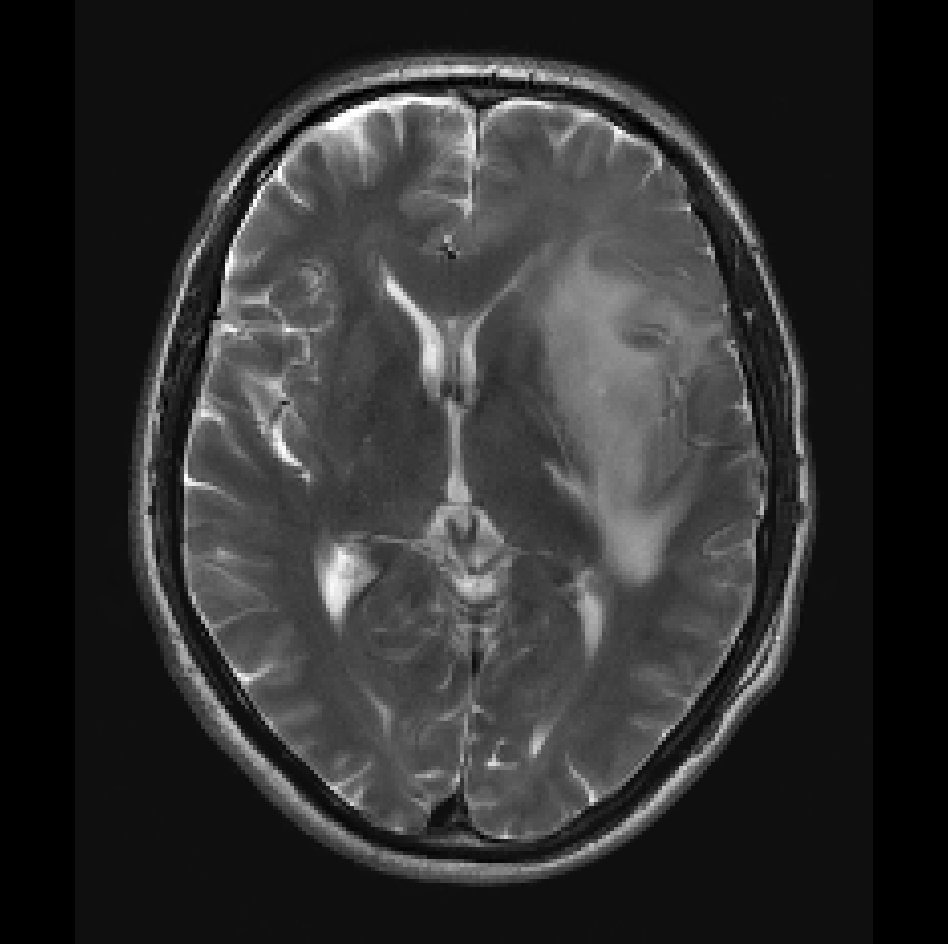
\includegraphics[width=\textwidth]{Figures/T2_LGG.png}
        \caption{Modern glioma scan}\label{fig:intro_MR_modern}
    \end{subfigure}
    \caption{\acrshort{MRI} scan of a glioma from 1980 and a recent \acrshort{MR} scan, showing the large improvement over time. On the modern scan the glioma can easily be identified}\label{fig:intro_MR_comparison}
\end{figure}
